
\section{Shadow Mapping}

Shadow Mapping is a image-based shadowing technique.

% The technique was first described in \cite{lance78}.

In 1985, Pixar used shadow mapping to create the video Luxo Jr. This
non real-time video was extremely impressive at its time. Especially
because of the shadows. 16 years later, in 2001 at Macworld Expo
Japan, Steve Jobs shows a real-time version of Luxo Jr. with the
exact same scene rendered using OpenGL.

In figure \ref{fig:scene} a small scene rendered without shadows can
be seen. Later when shadow mapping have been added, it is clear to see
how much difference simple shadows make.

\begin{figure}[h]
  \centering
  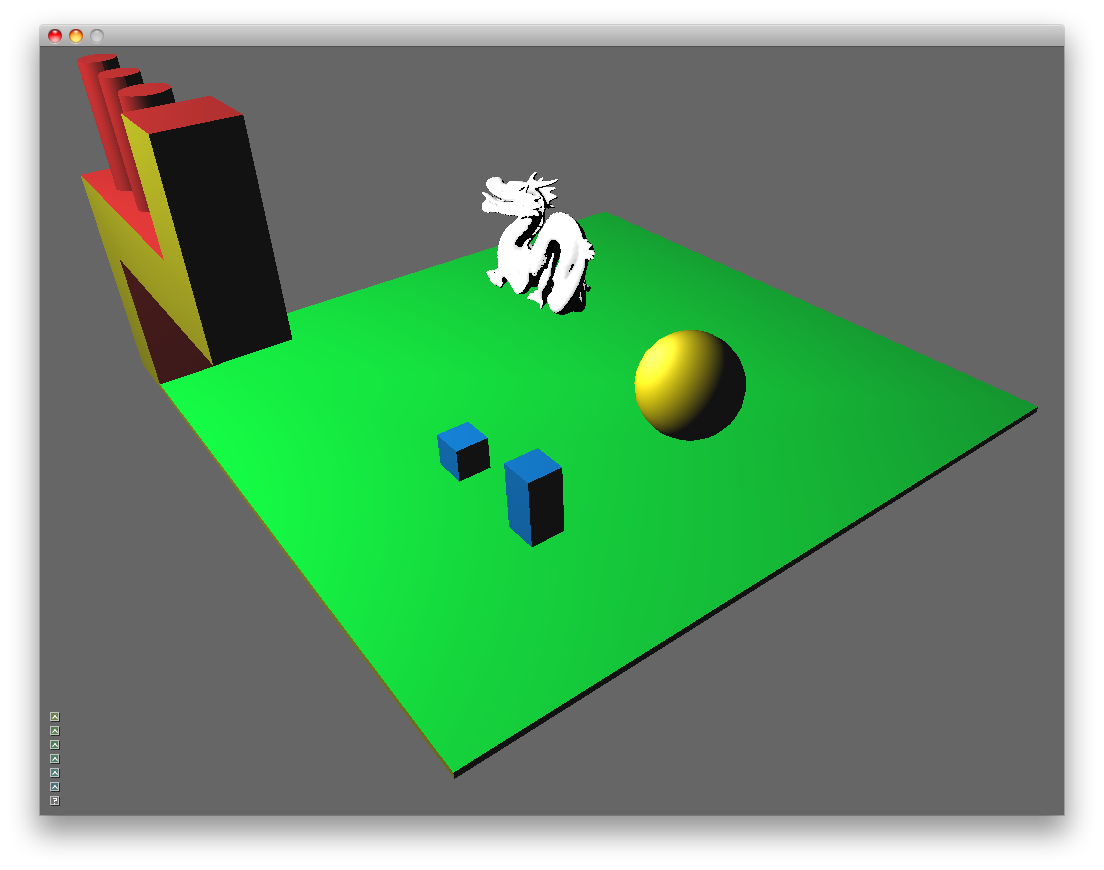
\includegraphics[width=\textwidth]{gfx/scenenoshadow}  
  \caption{Scene Without Shadows}
  \label{fig:scene}
\end{figure}

Shadow Mapping is a two-pass algorithm. The first step is to create
the ``Shadow Map'' which describes the scene from the light sources
point of view. In the second pass this map will be used to add shadows
while rendering the scene as seen by the camera.


\subsection{The light source}

To create the shadow map, the light sources need a bit more
information than usually. Regular lights in OpenGL have properties
that describes the amount of light emitted, and the placement of the
light source. This is not enough, as we need to create a project to be
able to render the scene from the light. \todoPtx{omskriv?}

Because of this, a light sources is more like a camera, which gives us
a nice abstraction. \todoPtx{complete me}


\subsection{Creating the Shadow map}

The first part of the algorithm is to create the shadow map. This is
done by rendering the scene using the light source as the camera, and
extracting the depth buffer.

\todoPtx{Husk at implementere det} The only interesting information is
the depth, so the rendering can be speed up be disabling textures,
lighting, colors and more. Its also convenient to disable front faces
to avoid self-shadowing. % bla bla?

\begin{figure}[h]
  \centering
  
\includegraphics[width=\textwidth]{gfx/shadowmap}  
  \caption{Shadow Map}
  \label{fig:shadowmap}
\end{figure}

In figure \ref{fig:shadowmap}, the shadow map for the scene in figure
\ref{fig:scene} is shown.

\subsection{Rendering the Scene}


The next step is to render the scene with shadows. For each fragment
in the finished scene, we must decide if it is in a shadow or
not. This is done by comparing the depth of the fragment with depth in
the shadow map.

%\subsubsection{Lookup in the shadow map}

Before we can compare anything, we need to find the corresponding
point in the shadow map. To calculate this, we need create a
projection matrix that converts model coordinates into projective
texture coordinates.

The first step is to convert model space to world space, this is done
using the regular modeling matrix ($M$)that we also use for rendering
the scene. The next step is to convert this to light space, using the
lights view matrix ($V_{light}$). We convert this to screen space via
the lights projection matrix ($P_{light}$). This will give us a
coordinate in the $[-1,1] \times [-1,1]$ range. This is a problem, as
texture space is in the range $[0,1] \times [0,1]$, so we add a bias
matrix ($B$), that does this conversion.

\begin{align*}
  B &= \begin{bmatrix}
    \frac{1}{2} & 0   & 0   & \frac{1}{2} \\
    0   & \frac{1}{2} & 0   & \frac{1}{2} \\
    0   & 0   & \frac{1}{2} & \frac{1}{2} \\
    0   & 0   & 0   & 1   \\
  \end{bmatrix} \\
  T &= BP_{light}V_{light}M
\end{align*}

%\subsubsection{Comparing Depth}

Once we have the right point, all there is left is to compare the
depth of the shadow map, and the coordinates $z$-component. When the
value in the shadow map is largest, it means that something is closer
to the light source, than the fragment we are processing.

\todoPtx{Kunne skrives bedre...}
Now we know if the fragment is in shadow, and change the color
to visualise it.

\begin{figure}[h]
  \centering
  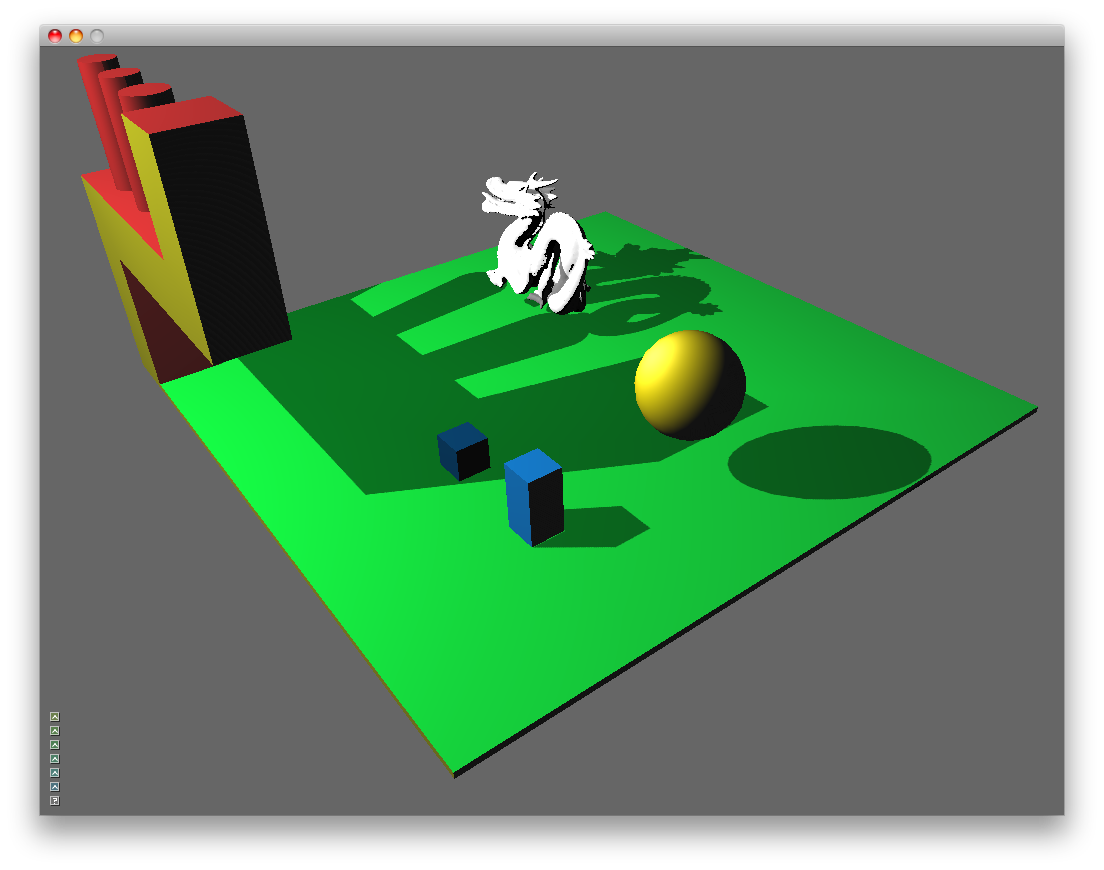
\includegraphics[width=\textwidth]{gfx/scenewithshadow}  
  \caption{Scene with shadows}
  \label{fig:sceneshadow}
\end{figure}

In figure \ref{fig:sceneshadow}, the scene is rendered using a single
shadow map.


%% -------------


\subsection{Implementation}

Our implementation of shadow mapping is based on OpenGL 2.1 with
shader language 1.20, and the framebuffer extension
(\texttt{GL\_ARB\_framebuffer\_object}).

\subsubsection{Lighting}

When we add vertex and fragment shaders to our pipeline, we loose all
the fixed functions, so we need to implement our own lighting.

\subsection{Limitations}



Shadow mapping is a technique for adding shadows in projection based \todoPtx{fixy?}
3D rendering. As such, it is limited by what is possible with projections.

One of these is that we cant have a field of view larger than 180
degrees\todoPtx{reference}. Therefor shadow mapping wont work with point
light sources.

%%% Local Variables: 
%%% mode: latex
%%% TeX-master: "master"
%%% End: 
